\ifdefined\ANONBUILD
\documentclass[sigconf,anonymous,review]{acmart}
\else
\documentclass[sigconf,review]{acmart}
\fi

\usepackage{amsmath}
\usepackage{booktabs}
\usepackage{placeins}
\usepackage{tabularx}
\newif\ifanonymoussubmission
\ifdefined\ANONBUILD
  \anonymoussubmissiontrue
\else
  \anonymoussubmissionfalse
\fi

\newcommand{\system}{TRACE-RPG}
\newcommand{\Valid}{\mathrm{valid}}
\newcommand{\AcceptSet}{\mathcal{A}}
\newcommand{\GoalSet}{\mathcal{G}}
\newcommand{\HitSet}{\mathcal{H}}
\newcommand{\SchemaSet}{\mathcal{S}}
\newcommand{\RepoURL}{\ifanonymoussubmission [Anonymous Repository URL withheld for double-anonymous review]\else \url{https://github.com/akillness/neural_symbolic_in_game}\fi}
\AtBeginDocument{\emergencystretch=2.5em}
\providecommand{\Description}[2][]{}


\setcopyright{none}
\acmConference[FDG '27]{Foundations of Digital Games}{2027}{\ifanonymoussubmission Anonymous Submission\else Seoul, Republic of Korea\fi}

\begin{document}

\title{TRACE-RPG: Auditable Proposal-to-Commit Boundaries and Deterministic Engine Verification for Interactive Games}

\author{Jangyoung Jeong}
\affiliation{\institution{Department of Game Design, Hongik University}\city{Seoul}\country{Republic of Korea}}
\author{Shinjin Kang}
\authornote{Corresponding author.}
\affiliation{\institution{Hongik University}\city{Seoul}\country{Republic of Korea}}

\begin{abstract}
Generated game events can satisfy a syntactic schema and cite known facts while requesting inaccessible objects, unauthorized state transitions, or premature secret disclosure. \system{} separates proposal authority from commit authority via a deterministic seven-predicate gate, counterexample-guided repair $\rho$, and hash-linked replay integrated with Godot~4.7.1, formalized by Theorems~1--4. Across 1,664 finite-graph cases, semantic gating eliminated 260/416 unsafe commits (0/156 false rejections; 128/260 repairs); across five quest worlds (120 closure cases), \texttt{multihop\_}\allowbreak\texttt{ontology\_}\allowbreak\texttt{gate} achieves 100.0\% accuracy vs.\ 50.83\% flat rules ($p{<}10^{-16}$). Across 16 live Gemini-to-headless Godot~4.7.1 closed-loop episodes (+ 16 fresh 0-LLM replays), 0/16 secret leaks occurred with 16/16 replay parity (\texttt{gemini-4-}\allowbreak\texttt{hydrogen-\allowbreak medium} 8/8 \texttt{EXACT\_}\allowbreak\texttt{TERMINAL\_}\allowbreak\texttt{HASH}; \texttt{gemini-3.8-}\allowbreak\texttt{flash-\allowbreak medium} 5/8, 4 parse failures retained, plus one safe actor-ID refusal). Together with 30-episode 5-arm shielding (66.7\% vs.\ 33.3\% safe goals, $p{=}0.00195$), 60 live 5-world shielding tasks (12/12 zero-token $\rho$ vs.\ 2/12 LLM self-repair), 268 EN/KO escape checks (97.2--100.0\% recall, 0/72 FRR), and a concrete \texttt{TR01--TR06} packet (\texttt{AWAITING\_}\allowbreak\texttt{HUMAN\_}\allowbreak\texttt{RATERS}), these results establish reproducible engine-verified boundaries.
\end{abstract}

\begin{CCSXML}
<ccs2012>
   <concept>
       <concept_id>10010147.10010178.10010187</concept_id>
       <concept_desc>Computing methodologies~Knowledge representation and reasoning</concept_desc>
       <concept_significance>500</concept_significance>
   </concept>
   <concept>
       <concept_id>10011007.10011074.10011099</concept_id>
       <concept_desc>Software and its engineering~Software verification and validation</concept_desc>
       <concept_significance>300</concept_significance>
   </concept>
</ccs2012>
\end{CCSXML}

\ccsdesc[500]{Computing methodologies~Knowledge representation and reasoning}
\ccsdesc[300]{Software and its engineering~Software verification and validation}

\keywords{game AI, interactive narrative, neuro-symbolic systems, Godot, deterministic verification}

\maketitle

\section{Introduction}
Generated game events can satisfy a syntactic schema and cite known facts while requesting inaccessible objects, unauthorized state changes, or premature secret disclosure. Grounding and plausible dialogue \cite{S03_weir2024ontologically,S20_ashby2023personalized} supply candidate content, yet the game engine must still decide which state transitions to authorize.

\system{} enforces this decision at an external proposal-to-commit boundary (Fig.~\ref{fig:architecture}). Models and adapters submit typed candidates to a deterministic gate that checks action policies, preconditions, object reachability, NPC knowledge, disclosure permissions, effects, and quest-stage monotonicity. When a check fails, the gate returns structured errors for bounded repair; repair modifies only the candidate rather than canonical state, and mutation occurs only after same-state revalidation. A read-only eight-role ontology view links source declarations to these checks and public decisions without write authority, while hash-linked transition records support semantic replay and assignment-complete accounting.

Conceptually, this contract goes beyond factual grounding by separating an NPC's \emph{epistemic knowledge boundary} (facts an actor knows) from its \emph{disclosure authorization policy} (facts an actor may reveal at the current quest stage). Methodologically, our evaluation separates a zero-LLM-call deterministic verification layer (gate checks, guided repair, and engine replay) from a bounded stochastic proposer layer with explicit failure retention.

Across our deterministic audits, a schema-only baseline committed 260/416 reference-invalid proposals across 32 finite-graph configurations, whereas all semantic-gate arms recorded 0/416 unsafe commits while preserving 156/156 valid proposals ($0/156$ false rejections) and 11/11 structural signatures; guided repair recovered 128/260 invalid proposals. In single-hop disclosure checks, general-rule and ontology-gate implementations agreed on 60/60 cases while eliminating 51 unique unsafe disclosures from an unchecked baseline; a subsequent 48-case multi-hop closure benchmark separates them cleanly (\texttt{ontology\_}\allowbreak\texttt{multihop\_}\allowbreak\texttt{gate} 48/48 vs.\ \texttt{flat\_}\allowbreak\texttt{1hop\_}\allowbreak\texttt{rule} 20/48, preventing 28 leaks). Extended zero-LLM audits, Theorems~1--4 for invariants \textbf{I1--I4}, a 24-episode live multi-quest Gemini evaluation (2/2 models, 3 worlds, 0 unsafe commits, 24/24 strict replay), Stage-2 EN/KO escape verifiers (97.2\% paraphrase recall at 0.0\% benign false rejection), and a trace-bound 36-item human-evaluation packet (\texttt{AWAITING\_}\allowbreak\texttt{HUMAN\_}\allowbreak\texttt{RATERS}) with Croissant~1.0 metadata complete our reproducible release boundary.

\section{Related Work and Research Gap}
Grounding, memory, planning, and role-based agents \cite{S03_weir2024ontologically,S20_ashby2023personalized,S07_park2023generative,S08_shao2023character}, together with player and dialogue systems \cite{S21_akoury2023player,S22_hochreiter2026beyond,S23_yin2026contextualized,S02_figueiredo2025scaffolded}, support contextual interaction, whereas we examine whether the current encoded state and disclosure policy permit a proposed transition. Modeling affect and engagement \cite{S24_yannakakis2011experiencedriven,S25_melhart2020engagement,S26_wang2026engagement} targets different outcomes: style preferences, affect estimates, and personality labels may guide generation but do not authorize state mutations.

Existing benchmarks and automated play-testing cover state, embodiment, content, process, social interaction, and long-horizon play \cite{S11_cote2019textworld,S12_wang2022scienceworld,S13_fan2022minedojo,S14_perezliebana2019gvgai,S15_liu2024agentbench,S16_ma2024agentboard,S17_zhou2024sotopia,S18_paglieri2025balrog,S19_lepelletier2022playtesting}, while NCP-Bench evaluates narrative commitment and fact consistency \cite{S58_ma2026ncpbench}. Structural, schema, affordance, and neuro-symbolic rule methods motivate our constraint design \cite{S09_geng2023grammar,S10_beurerkellner2023prompting,S36_scholak2021picard,S50_kambhampati2024llmmodulo,S51_ichter2023saycan,S52_wang2025agentspec,S53_li2025settingdc,S54_zhou2025story2game,S42_buongiorno2024pangea}, alongside counterexample-guided repair \cite{S45_madaan2023selfrefine,S48_shinn2023reflexion,S46_chen2023selfdebug,S47_solarlezama2006sketching} and reproducibility/accounting standards \cite{S31_agarwal2021precipice,S33_pineau2021reproducibility,S56_feng2025agentrr,S59_sun2025bdc}. Unlike prior systems that conflate schema validity with action legality or treat factual grounding as sufficient for dialogue safety, \system{} isolates schema parsing, epistemic knowledge, disclosure permission, and canonical state commit into separately auditable gates.


\begin{figure*}[!t]
  \centering
  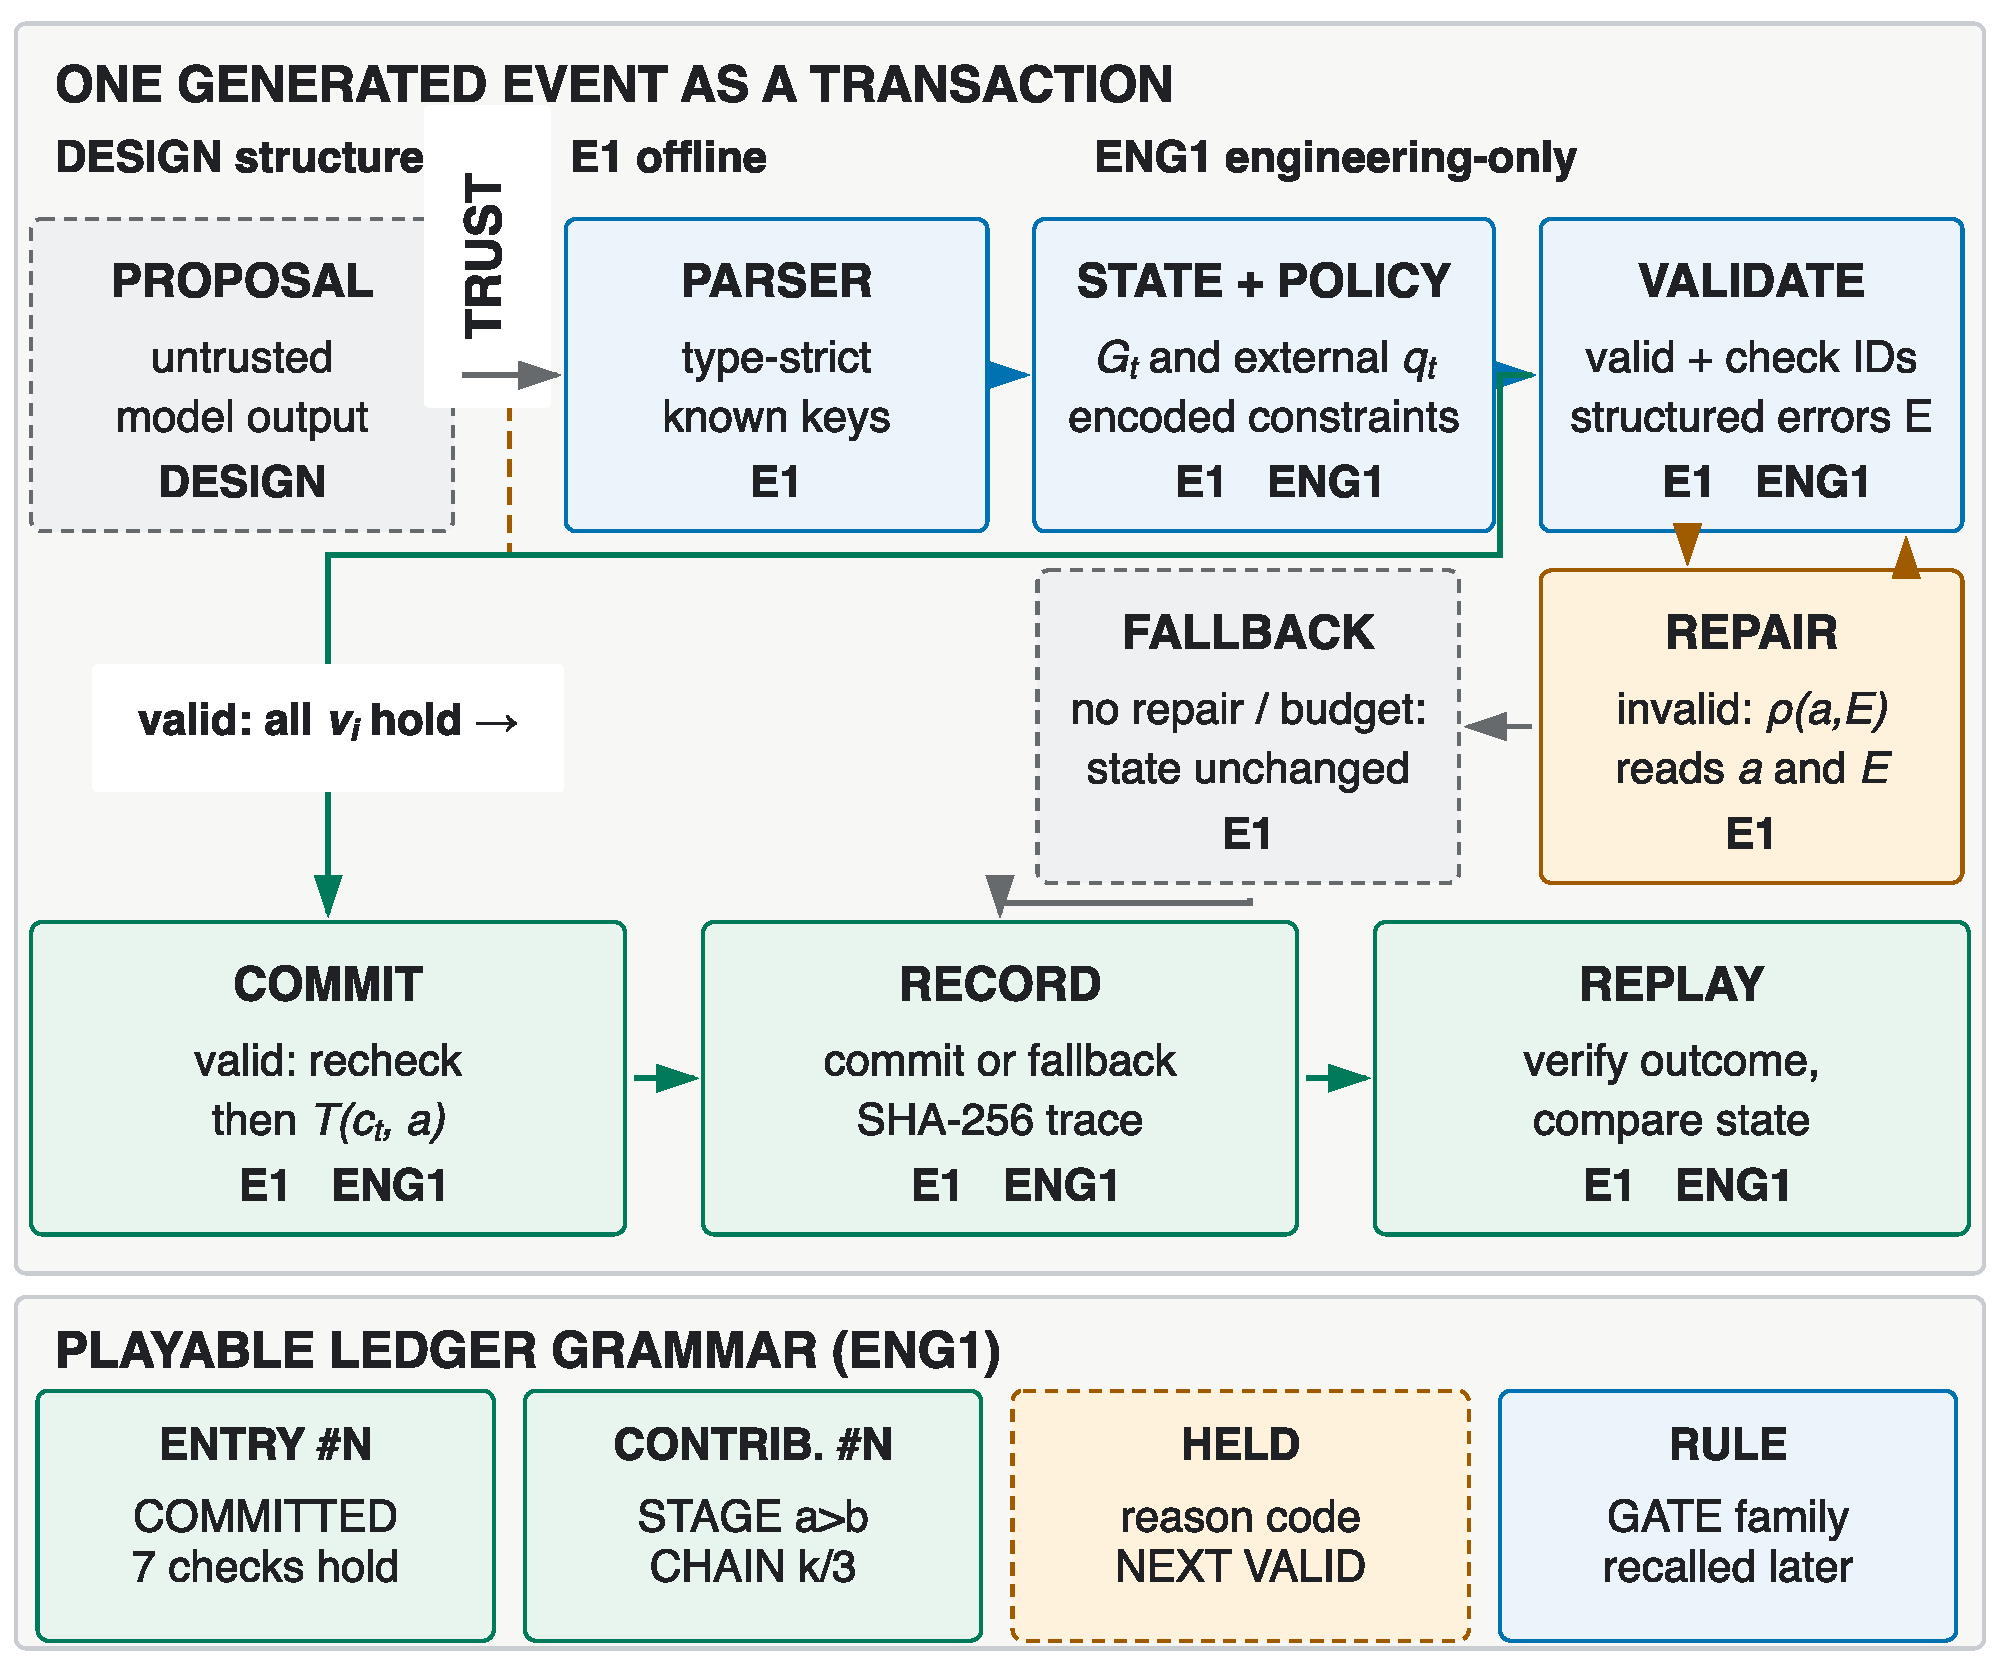
\includegraphics[width=0.72\textwidth]{../../figures/fig_architecture.pdf}
  \caption{Policy and state $c_t$ gate proposals; errors feed bounded $\rho$ or unchanged fallback before revalidated commit and replay.}
  \Description{Architecture diagram showing proposal submission, seven-predicate deterministic validation, bounded repair, revalidation, and commit ledger.}
  \label{fig:architecture}
\end{figure*}

\section{Problem Definition and Guarantee Boundary}\label{sec:problem}
In $c_t=(G_t,q_t)$, $G_t$ denotes the typed game snapshot (locations, reachable locations, object placements, inventory, facts, NPC knowledge, and quest stage) and $q_t$ contains externally authored action-policy, disclosure, and quest-stage constraints. Predicates neither reconstruct history $h_{<t}$ nor mutate $q_t$, and retrieval outputs or affect scores carry zero write authority.

After strict schema parsing of an untrusted proposal $a_t$, the validator runs seven deterministic predicates and returns \texttt{Validation}\allowbreak\texttt{Result}(\allowbreak$\mathrm{valid},E_t,C_{\mathrm{run}}$):
\begin{equation}
\begin{aligned}
V(c_t,a_t)&=(\mathrm{valid},E_t,C_{\mathrm{run}}),\\
\boldsymbol{v}&=(v_{\mathrm{policy}},v_{\mathrm{pre}},v_{\mathrm{reach}},\\
&\qquad v_{\mathrm{know}},v_{\mathrm{disc}},v_{\mathrm{elig}},v_{\mathrm{stage}})\in\{0,1\}^{7},
\end{aligned}
\end{equation}
where $\mathrm{valid}\equiv\bigwedge_{i=1}^{7}(v_i=1)$ and $E_t$ records typed error codes, entities, reasons, and repair hints. Canonical state updates only when all seven predicates pass:
\begin{equation}
c_{t+1}=\begin{cases}
T(c_t,a_t), & \bigwedge_{i=1}^{7}(v_i=1),\\
c_t, & \text{otherwise.}
\end{cases}
\label{eq:transition}
\end{equation}

\subsection{Schema Validity, Authorization, and Goal Success}\label{sec:authorization-sets}
Fix the pre-action state $c_t$, authored policy, and strict schema. Let $\SchemaSet$ be the set of schema-valid candidates; we separate authorization from goal attainment:
\begin{equation}
\begin{aligned}
\AcceptSet(c_t)&=\{a\in\SchemaSet:V(c_t,a).\mathrm{valid}\},\\
\GoalSet(c_t)&=\{a\in\SchemaSet:\operatorname{Goal}(T(c_t,a))\},\\
\HitSet(c_t)&=\AcceptSet(c_t)\cap\GoalSet(c_t)\subseteq\AcceptSet(c_t)\subseteq\SchemaSet.
\end{aligned}
\end{equation}
A schema-valid candidate that declares a forbidden fact falls outside $\AcceptSet$, whereas a permitted observation action can lie inside $\AcceptSet$ yet outside $\GoalSet$. Knowledge and disclosure permission are independent inputs: an NPC can know \texttt{keeper\_\allowbreak secret} at both stage $0$ and stage $1$ while disclosure is forbidden at stage $0$ and permitted at stage $1$.

\subsection{Formal Security Theorems for Invariants I1--I4}\label{sec:formal-proofs}
Under Eq.~\eqref{eq:transition} and strict parser \texttt{parse\_}\allowbreak\texttt{candidate\_}\allowbreak\texttt{mapping}, invariants \textbf{I1--I4} hold as conditional structural theorems over any finite encoded state $c_t=(G_t,q_t)$, repair budget $K\in\mathbb{Z}_{\geq 0}$, and returning callbacks:

\noindent\textbf{Theorem 1 (I1: State-Preservation Safety).} \emph{If the initial candidate fails strict parsing or all $K{+}1$ candidates yield $V(c_t,a^{(j)}).\mathrm{valid}=\mathrm{false}$, then $c_{t+1}=c_t$ and committed effects are empty.}
\par\noindent\textit{Proof.} \texttt{parse\_}\allowbreak\texttt{candidate\_}\allowbreak\texttt{mapping} rejects malformed proposals prior to commit; in Fig.~\ref{alg:commit}, $\operatorname{Commit}$ is reachable only on $\mathrm{ok}=\mathrm{true}$, while $j=K$ invokes $\operatorname{Fallback}(c_t)$ returning $c_t$ untouched by Eq.~\eqref{eq:transition}. \hfill$\square$

\noindent\textbf{Theorem 2 (I2: Bounded Termination and State-Blind Anti-Laundering Repair).} \emph{For any finite $K{\geq}0$ and returning callbacks, the loop executes at most $K{+}1$ validator calls, revalidates $V(c_t,a^{(j)})$ immediately prior to mutation, and never alters \texttt{WorldState}-dependent authorization classes under $\rho$.}
\par\noindent\textit{Proof.} Loop counter $j$ starts at $0$, checks $j=K$ before incrementing, and halts on $\mathrm{ok}=\mathrm{true}$ or $j=K$, bounding $V$ calls by $K{+}1$. By Table~\ref{tab:rho-rules}, $\rho(a,E)$ inspects only $(a,E)$ without reading \texttt{WorldState} and maps \texttt{UNKNOWN\_}\allowbreak\texttt{ACTION\_}\allowbreak\texttt{TYPE}, \texttt{UNREACHABLE\_}\allowbreak\texttt{REQUIRED\_}\allowbreak\texttt{OBJECT}, \texttt{NPC\_}\allowbreak\texttt{KNOWLEDGE\_}\allowbreak\texttt{VIOLATION}, \texttt{NPC\_}\allowbreak\texttt{DIS\-CLOSURE\_}\allowbreak\texttt{KNOW\-LEDGE\_}\allowbreak\texttt{VIO\-LATION}, \texttt{FORBIDDEN\_}\allowbreak\texttt{DISCLOSURE}, \texttt{QUEST\_}\allowbreak\texttt{STAGE\_}\allowbreak\texttt{VIOLATION}, and \texttt{QUEST\_}\allowbreak\texttt{STAGE\_}\allowbreak\texttt{REGRESSION} to identity while dropping same-field conflicts. \hfill$\square$

\noindent\textbf{Theorem 3 (I3: Policy-Bounded Mutation).} \emph{Every committed state transition satisfies all seven predicates $v_1\dots v_7$ and applies only effects permitted by \texttt{ActionPolicy.}\allowbreak\texttt{allowed\_}\allowbreak\texttt{effects}.}
\par\noindent\textit{Proof.} Strict parsing freezes the 12 \texttt{CANDIDATE\_}\allowbreak\texttt{FIELDS}; $v_{\mathrm{policy}}{=}1$ verifies effect membership in \texttt{allowed\_}\allowbreak\texttt{effects} and $T$ writes no undeclared keys. \hfill$\square$

\noindent\textbf{Theorem 4 (I4: Deterministic Semantic Replay).} \emph{Given ordered hash-chained transition records with \texttt{allow\_}\allowbreak\texttt{defaults=false} parsing and frozen $(V,T)$, replaying proposals from $c_0$ uniquely reconstructs $c_T$ and detects any single-step tampering via SHA-256 chain mismatch.}
\par\noindent\textit{Proof.} Both $V$ and $T$ are pure deterministic functions of $(c_t,a_t)$, and each record hashes $(\mathrm{hash}(c_t),\allowbreak a_t,\allowbreak V(c_t,a_t),\allowbreak\mathrm{hash}(c_{t+1}))$; inductive agreement from $c_0$ yields $\mathrm{hash}(c'_T)=\mathrm{hash}(c_T)$. \hfill$\square$

\section{TRACE-RPG Architecture and Algorithms}\label{sec:arch}
Models and adapters propose candidate actions, the strict parser rejects unknown keys and ambiguous types, and a versioned bridge carries observations, proposals, validations, rejections, fallbacks, and commits (Fig.~\ref{fig:architecture}, Table~\ref{tab:validators}). An eight-role read-only ontology view (\texttt{World}, \texttt{Actor}, \texttt{Knowledge}, \texttt{Fact}, \texttt{Policy}, \texttt{Quest}, \texttt{Action}, \texttt{Trace}) maps source declarations to executed checks and replay receipts without granting mutation authority.

\begin{table}[!tbp]
\caption{Encoded Seven-Predicate Validator Boundary}
\label{tab:validators}
\centering
\footnotesize
\begin{tabularx}{\columnwidth}{@{}>{\raggedright\arraybackslash}p{0.26\columnwidth}>{\raggedright\arraybackslash}X>{\raggedright\arraybackslash}p{0.18\columnwidth}@{}}
\toprule
\textbf{Predicate} & \textbf{Rejects} & \textbf{On failure} \\
\midrule
Action policy & unknown action/type; omitted required preconditions/effects; disallowed effects & unchanged \\
Precondition & absent or false requirement & unchanged \\
Reachability & inaccessible target object & unchanged \\
NPC knowledge & used/disclosed fact absent from actor knowledge & unchanged \\
Disclosure & declared forbidden fact & unchanged \\
Quest stage & required stage above current stage & unchanged \\
Stage monotonicity & regressive quest-stage mutation & unchanged \\
\bottomrule
\end{tabularx}
\end{table}

\begin{figure}[!tbp]
\centering
\footnotesize
\begin{tabular}{@{}rl@{}}
1: & $a\leftarrow\operatorname{Propose}(c)$; $j\leftarrow0$ \\
2: & \textbf{repeat} \\
3: & \quad $(\mathrm{ok},E)\leftarrow V(c,a)$; $\operatorname{Record}(a,E)$ \\
4: & \quad \textbf{if} $\mathrm{ok}$ \textbf{then assert} $V(c,a).\mathrm{ok}$; \textbf{return} $\operatorname{Commit}(c,a)$ \\
5: & \quad \textbf{if} $j=K$ \textbf{then return} $\operatorname{Fallback}(c)$ \\
6: & \quad $a\leftarrow\operatorname{Repair}(c,a,E)$; $j\leftarrow j+1$ \\
7: & \textbf{until terminal}
\end{tabular}
\caption{Validate--Repair--Commit records at most $K+1$ candidate attempts and revalidates before mutation.}
\Description{Pseudocode of the Validate-Repair-Commit loop bounding validator calls to K+1 and revalidating prior to commit.}
\label{alg:commit}
\end{figure}

The guided repair operator $\rho(a,E)=a\oplus\bigcup_{e\in E}\delta(e)$ (Fig.~\ref{alg:commit}, Table~\ref{tab:rho-rules}) receives only candidate $a$ and structured errors $E$, never \texttt{WorldState}, preventing state laundering on reachability, knowledge, or disclosure violations. Transition records chain unkeyed SHA-256 hashes over prior state, candidate, validation outcome, and recomputed final state for deterministic semantic replay and assignment-complete denominator accounting.

\begin{table}[!tbp]
\caption{Per-Error-Class Edits of Guided Repair $\rho(a,E)$}
\label{tab:rho-rules}
\centering
\footnotesize
\begin{tabularx}{\columnwidth}{@{}>{\raggedright\arraybackslash}X>{\raggedright\arraybackslash}X@{}}
\toprule
\textbf{Validator error class} & \textbf{Edit $\delta(e)$ on candidate $a$} \\
\midrule
Policy precondition / effect omission & insert named predicate or effect \\
Policy effect violation & drop disallowed effect \\
Unsatisfied precondition & drop named predicate \\
Unauthorized stage mutation & clear \texttt{quest\_stage\_effect} \\
Unknown action; reachability, knowledge, disclosure, or stage classes & no-op (prevents state laundering) \\
\bottomrule
\end{tabularx}
\end{table}

\section{Evaluation}\label{sec:eval}
We separate zero-LLM-call deterministic audits from bounded stochastic proposer pilots; cohorts and denominators are never pooled across lanes.

\subsection{E1 Offline Conformance and Deterministic Boundary Audit}
In \textbf{E1} (13 gate fixtures and 12 repair cases per arm), all four arms satisfy construction invariants (13/13 gate agreement, 10/10 integrity fault detections). On invalid repair fixtures, \texttt{rejection\_only} and \texttt{unchanged\_retry} recover 0/12, guided repair $\rho$ recovers 5/12 without reading \texttt{WorldState}, and the nondeployable state-reading oracle recovers 6/12.

To test authorization beyond single-world fixtures, our deterministic boundary audit crosses two room counts (4, 8), two topologies (locked chain, unlocked bypass branch), four start/goal placements of two reusable keys, and two quest stages ($2{\times}2{\times}4{\times}2=32$ configurations) with 13 candidate variants each (416 assignments/arm; 1,664 total) plus 48 surface-sentinel assignments (12/arm). An implementation-separated reference evaluates initial and repaired candidates against the immutable pre-action state using standard-library BFS reachability.

\begin{table}[!tbp]
\caption{Deterministic Authorization-Boundary Audit (416 Cases/Arm + 48 Surface Sentinels; 0 LLM Calls)}
\label{tab:boundary-full}
\centering
\footnotesize
\begin{tabularx}{\columnwidth}{@{}>{\raggedright\arraybackslash}X*{4}{>{\centering\arraybackslash}p{0.125\columnwidth}}@{}}
\toprule
\textbf{Outcome (416/arm)} & \textbf{Schema only} & \textbf{Sem.\ reject} & \textbf{Unch.\ retry} & \textbf{Guided $\rho$} \\
\midrule
Invalid initial proposals & 260 & 260 & 260 & 260 \\
Unsafe final commits & 260 & \textbf{0} & \textbf{0} & \textbf{0} \\
Repaired invalid $\rightarrow$ valid & 0 & 0 & 0 & \textbf{128} \\
Held (unchanged fallback) & 0 & 260 & 260 & 132 \\
Goal reached & 124 & 124 & 124 & \textbf{252} \\
Valid preserved (156 valid) & 156 & 156 & 156 & 156 \\
Signature retention (11 sigs) & 11/11 & 11/11 & 11/11 & 11/11 \\
\bottomrule
\end{tabularx}
\end{table}

Table~\ref{tab:boundary-full} shows that \texttt{schema\_only} committed all 260/416 reference-invalid proposals, whereas every semantic-gate arm recorded 0/416 unsafe commits, 0/156 false rejections, and 32/32 closure--BFS agreement. Guided repair $\rho$ recovered 128/260 invalid proposals, raising goal attainment from 124/416 to 252/416. On the 12/arm surface sentinels, all semantic gates blocked 6/6 explicit forbidden-fact declarations but admitted 6/6 undeclared paraphrases, quantifying the declared-field boundary.

\subsection{Disclosure Parity, NPC Screening, and KG Simulation}
On 60 authored \texttt{reveal\_hint} cases (48 normal, 4 boundary, 8 malformed; Fig.~\ref{fig:disclosure-signals}), an unchecked baseline produced 51 unique unsafe disclosures (60/60 allow), whereas \texttt{general\_rule} and \texttt{ontology\_gate} agreed on 60/60 outcomes (16 allow, 44 deny, 0 unsafe, 0 replay mismatches), establishing zero-regression audit binding rather than ontology superiority. Separately, deterministic \texttt{NPC-ENG1} (16 cases) and historical \texttt{NPC-SCR1} (72 rows; 24/arm, 20/24 complete, 4/24 goal, 12 stale-control ACK rejections) verify protocol state transitions and replay. In the closed-world KG link-proposal simulation (43 OKF nodes, 106 reference edges, 24 curated typed edges, 6 withheld-edge queries), typed-lexical retrieval (\texttt{S2}) achieved $P{=}R{=}1.000$, $\mathrm{MRR}{=}0.944$, and $\mathrm{Sem@3}{=}1.000$ versus degree baseline $P{=}R{=}0.000$ and $\mathrm{MRR}{=}0.282$.

\begin{figure}[!tbp]
\centering
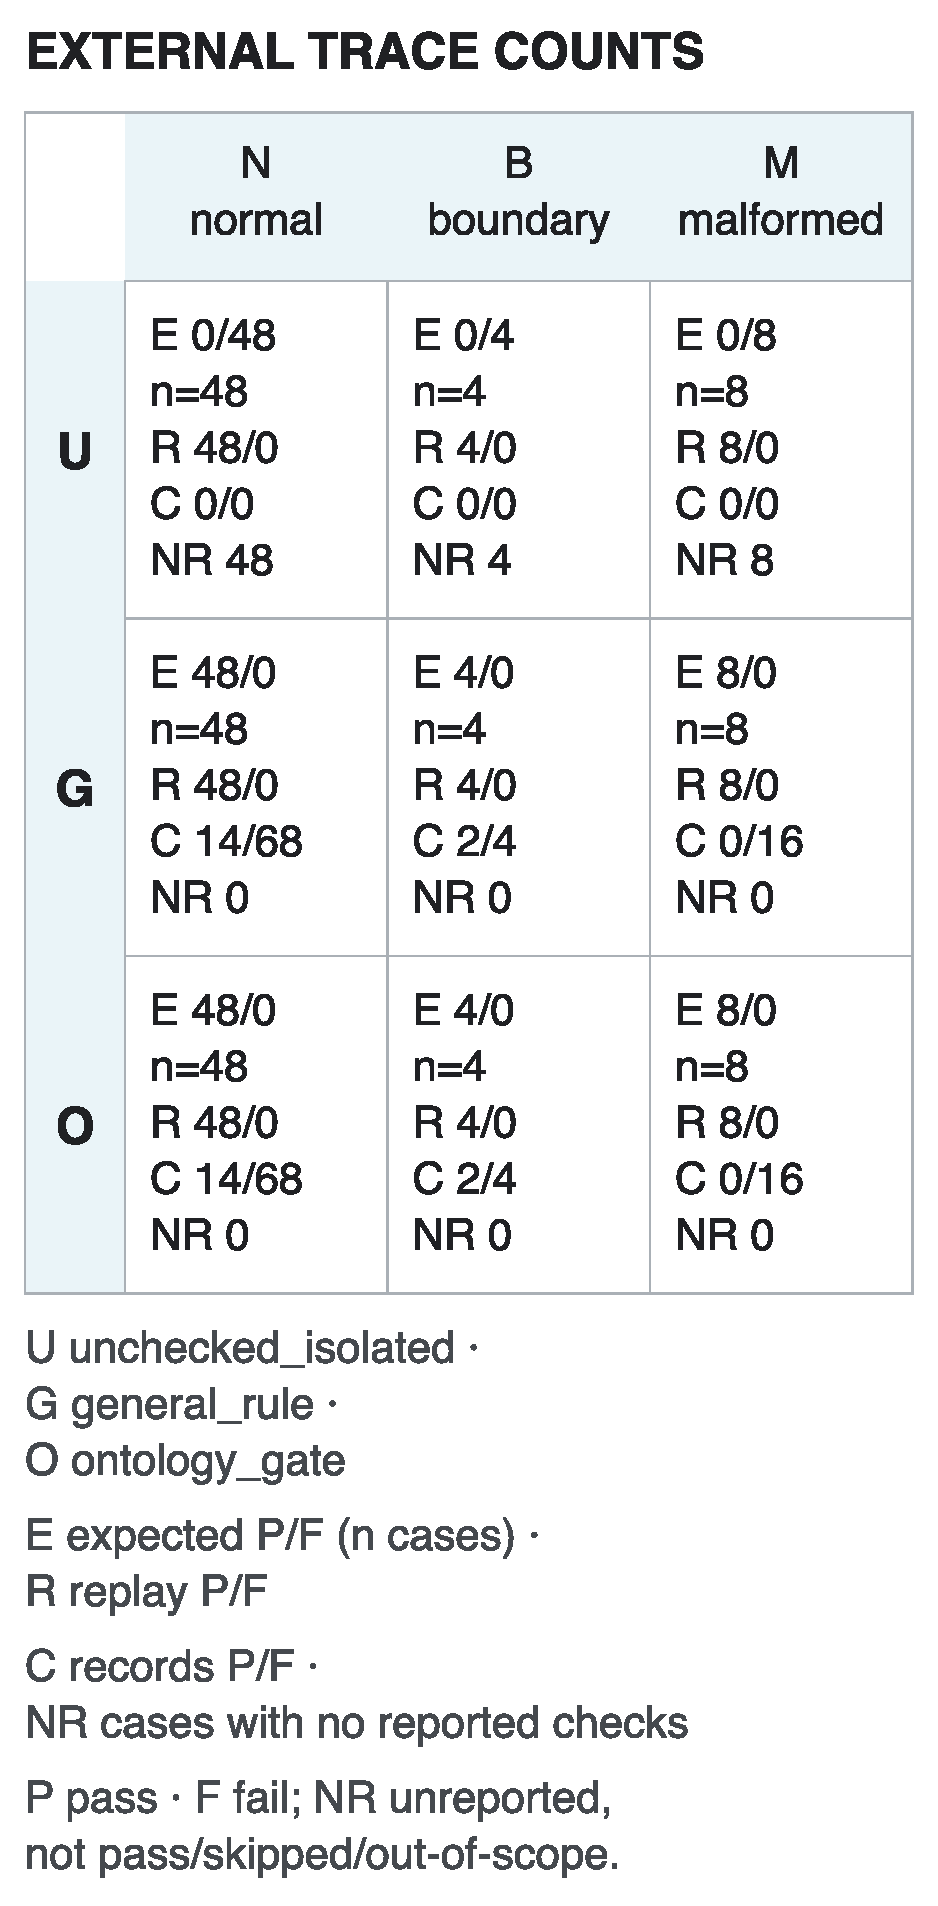
\includegraphics[width=\columnwidth]{../../figures/fig_disclosure_signals.pdf}
\caption{NPC-DISC-1 counts by arm and stratum (E/R: expectation match and replay; C: policy check PASS/FAIL; NR: no reported check).}
\Description{Bar matrix of NPC-DISC-1 counts by experimental arm and stratum comparing expectation match, replay, policy PASS/FAIL, and unreported checks.}
\label{fig:disclosure-signals}
\end{figure}

\subsection{Extended Zero-LLM Engineering Audits (A1--A4, B)}
Table~\ref{tab:extended-full} summarizes five independent-denominator deterministic audits covering multi-error repair convergence, latency scaling, seeded traceability sensitivity, Godot~4.7.1 soak stability (Fig.~\ref{fig:engine-cutscenes}), and secondary escape filtering.

\begin{table*}[!tbp]
\caption{Independent-Denominator Zero-LLM Engineering Audits (A1--A4, B)}
\label{tab:extended-full}
\centering
\footnotesize
\begin{tabularx}{\textwidth}{@{}>{\raggedright\arraybackslash}p{0.20\textwidth}>{\raggedright\arraybackslash}p{0.21\textwidth}>{\raggedright\arraybackslash}X@{}}
\toprule
\textbf{Audit} & \textbf{Denominator / Scope} & \textbf{Verified Deterministic Results (0 LLM Calls)} \\
\midrule
\textbf{A1} Multi-Error Convergence & 352 cases/budget ($K{\in}\{0..3\}$, 1,408 runs) + 128 guards & Safe commits: $K{=}0$ 0/352, $K{\ge}1$ 124/352 (35.23\%, unsafe 0/1,408); \texttt{repairable\_multi} 96/96 at $K{=}1$; \texttt{mixed\_partial\_clear} 28/160 at $K{=}1$, 132/160 held; \texttt{conflict\_pair} 0/96 cross-attempt commits (96/96 period-2 oscillation at $K{=}3$) vs.\ 128/128 same-pass conflict-guard freeze. \\
\textbf{A2} Scaling Benchmark & $N{\in}[10,2000]$ facts ($\text{arity}{\le}100$ above 500), $R{\in}[4,256]$ rooms & At $N{=}2000$: validator p95 0.0042\,ms (valid) / 0.0751\,ms (multi-error); $\rho$ p95 0.0317--0.0389\,ms; $R{=}256$ closure/BFS p95 0.312--0.478\,ms; SHA-256 verify 7.01\,ms; JSONL replay ($N{=}100,L{=}100$) 881.0\,ms. \\
\textbf{A3} Traceability Faults & 4,656 seeded faults (+1,584 N/A), 3,744 invariance, \texttt{TR05} map & Seeded sensitivity 4,656/4,656 (100.00\%); invariance false alarms 0/3,744 (0.00\%); \texttt{TR05} forward 12/12, reverse 10/10 direct files; human Krippendorff $\alpha$ unmeasured (0 human raters). \\
\textbf{A4} Godot~4.7.1 Soak & 11 refusals + 1,600 ticks (200 episodes) & Refusal codes 9/9 (100\%) exercised; state isolation 11/11; trace consistency 1,600/1,600; \texttt{step\_commit} p95 0.708\,ms; static memory delta $-268$\,B; 0 leaks. \\
\textbf{B} Escape Filter (EN/KO) & 88 cases (44 EN, 44 KO; \texttt{keeper\_secret}) & Recall / benign FRR / warm p95: ID-only 0.0\% / 0.0\% / 0.032\,ms; Alias 61.1\% (22/36) / 11.1\% (4/36) / 0.041\,ms; LOO TF-IDF 97.2\% (35/36) / \textbf{58.3\% (21/36)} / 0.705\,ms. \\
\bottomrule
\end{tabularx}
\end{table*}

\begin{figure*}[!tbp]
\centering
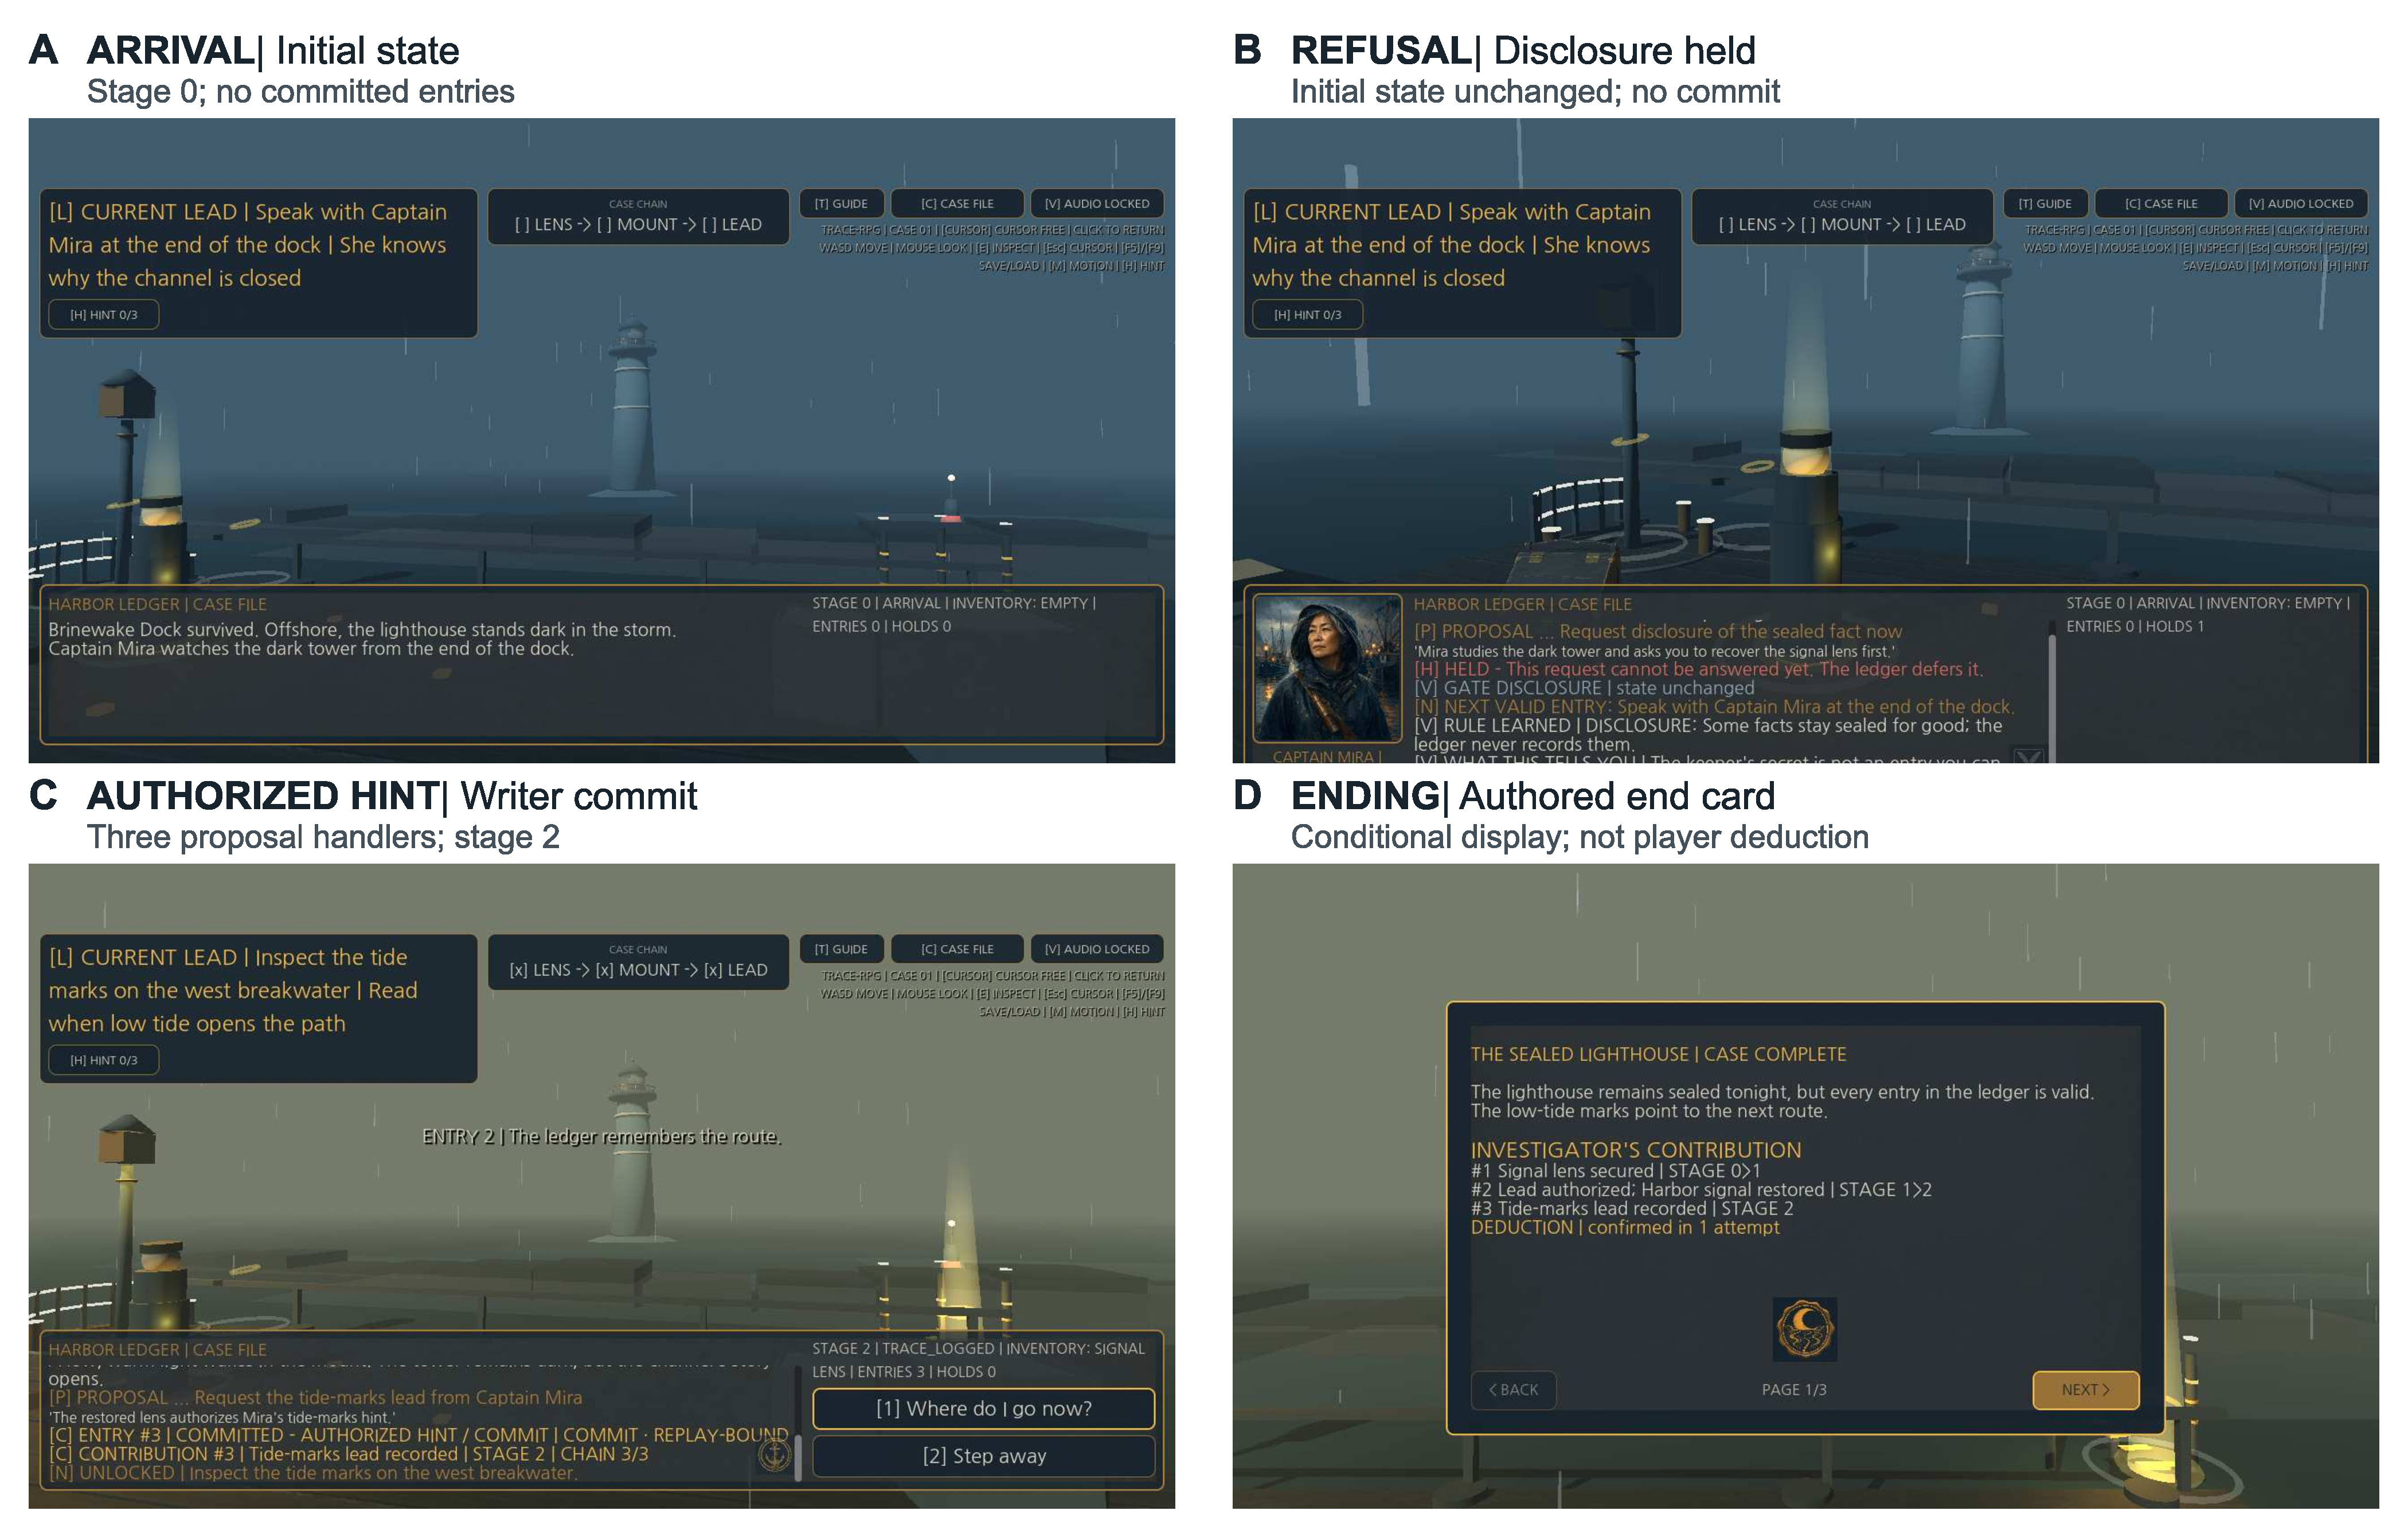
\includegraphics[width=0.92\textwidth]{../../figures/fig_engine_cutscenes.pdf}
\caption{Native Godot~4.7.1 engineering captures: (A) initial arrival; (B) denied secret disclosure leaving state unchanged; (C) authorized hint at stage 2; (D) conditional closing card. These captures verify rendered state correspondence rather than user efficacy.}
\Description{Four-panel Godot 4.7.1 screenshot sequence showing initial arrival, denied secret disclosure with unchanged state, stage-2 authorized hint, and closing card.}
\label{fig:engine-cutscenes}
\end{figure*}

\subsection{Bounded Stochastic Proposer Pilots}
In the \textbf{v5 two-stage collection} (20 assignments: 5 synthetic fixtures $\times$ 2 selectors $\times$ Detailed/Generic, $K{=}0$), 20/20 responses arrived, 10/20 passed strict parsing (Luna 9/10; Terra 1/10), 8/20 passed the semantic gate (Table~\ref{tab:v5-summary}, Fig.~\ref{fig:paired-feedback-flow}), and 7/20 reached \texttt{signal\_restored}; all 2 rejected parsed candidates fell back with zero state mutation. In the \textbf{native fixed-quest pilot} (8 assignments on \texttt{sealed-\allowbreak lighthouse-\allowbreak v1}), 5/8 reached the goal with 0/16 unsafe commits, 7/7 semantic replays valid, and 6/6 committed fresh Godot re-executions valid (1 pre-response controller-v3 serialization fault fixed to v4 in rows 2--8; 2 ontology rows timed out at 60\,s).

\begin{table}[!tbp]
\caption{v5 Synthetic Collection (5 Assigned Cases/Cell; Failures Retained)}
\label{tab:v5-summary}
\centering
\footnotesize
\begin{tabularx}{\columnwidth}{@{}ll*{4}{>{\centering\arraybackslash}X}@{}}
\toprule
\textbf{Selector} & \textbf{Signal} & \textbf{Recv} & \textbf{Gate} & \textbf{Goal} & \textbf{Parse Fail} \\
\midrule
\texttt{gpt-5.6-luna} & Detailed & 5/5 & 4/5 & 3/5 & 1/5 \\
\texttt{gpt-5.6-luna} & Generic  & 5/5 & 3/5 & 3/5 & 0/5 \\
\texttt{gpt-5.6-terra} & Detailed & 5/5 & 0/5 & 0/5 & 5/5 \\
\texttt{gpt-5.6-terra} & Generic  & 5/5 & 1/5 & 1/5 & 4/5 \\
\bottomrule
\end{tabularx}
\end{table}

\begin{figure}[!tbp]
\centering
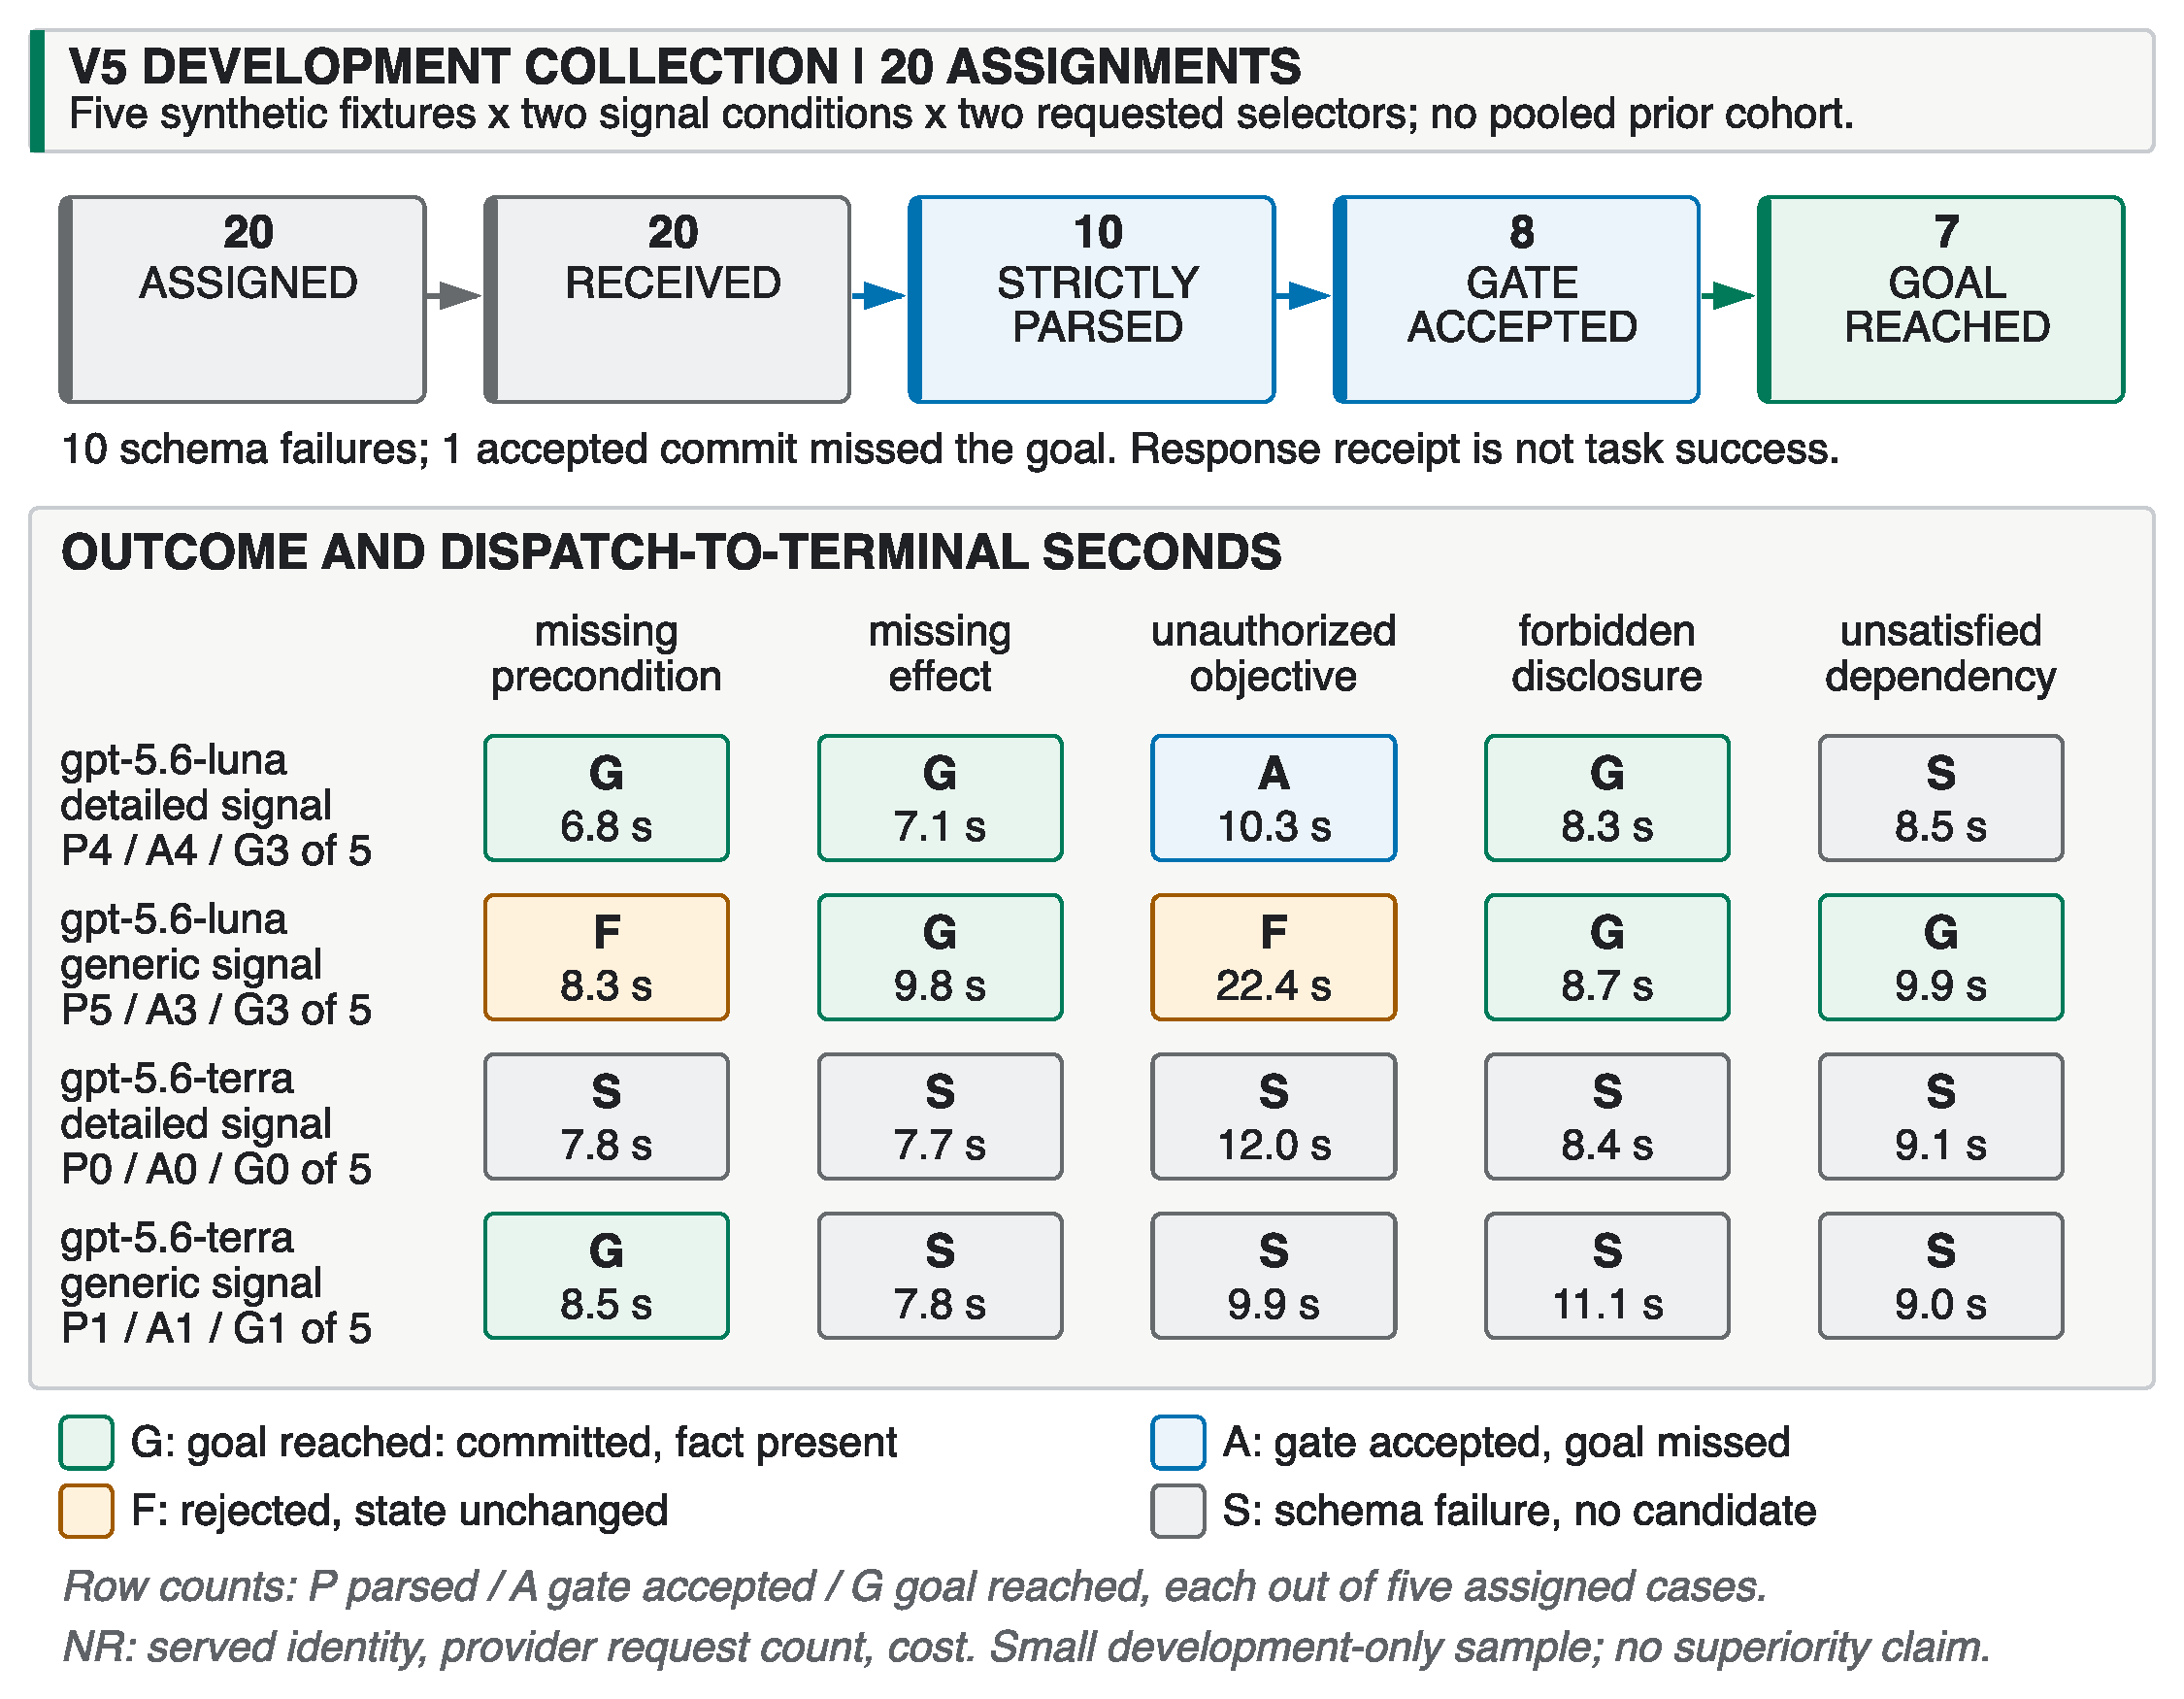
\includegraphics[width=\columnwidth]{../../figures/fig_paired_feedback_flow.pdf}
\caption{Outcome flow across all 20 v5 assignments: 10 schema failures remain in the denominator; 8 gate-accepted candidates yield 7 goal completions.}
\Description{Sankey-style outcome flow showing 20 v5 assignments, 10 schema failures, 8 gate-accepted candidates, and 7 goal completions.}
\label{fig:paired-feedback-flow}
\end{figure}

\subsection{Multi-Hop Ontology Closure (48 Cases Across Three Worlds)}\label{sec:multihop-eval}
While our 60-case single-hop disclosure check established zero-regression parity (\texttt{general\_rule} $=$ \texttt{ontology\_gate}), real narrative worlds require transitive role inheritance and fact-derivation chains. Across three deterministic quest worlds (\texttt{sealed-}\allowbreak\texttt{lighthouse-}\allowbreak\texttt{v1}, \texttt{sunken-}\allowbreak\texttt{archive-}\allowbreak\texttt{v1}, \texttt{clockwork-}\allowbreak\texttt{observatory-}\allowbreak\texttt{v1}), we constructed 48 evaluation cases balanced across 1-hop (16), derivation-chain (16), and role-inheritance (16) strata (37 unsafe disclosures/actions, 11 permitted). Table~\ref{tab:multihop-ontology} shows that \texttt{flat\_}\allowbreak\texttt{1hop\_}\allowbreak\texttt{rule} attains only 41.7\% accuracy (9 TP, 11 TN, 28 unsafe false-negative leaks, 0 FP), whereas \texttt{ontology\_}\allowbreak\texttt{multihop\_}\allowbreak\texttt{gate} achieves 100.0\% accuracy (37 TP, 11 TN, 0 FN, 0 FP), eliminating 28 leaks while passing \textbf{I1--I4} checks across all three worlds.

\begin{table}[!tbp]
\caption{Multi-Hop Epistemic and Disclosure Closure Benchmark (48 Cases Across 3 Quest Worlds)}
\label{tab:multihop-ontology}
\centering
\footnotesize
\setlength{\tabcolsep}{3.5pt}
\begin{tabularx}{\columnwidth}{@{}>{\raggedright\arraybackslash}X*{5}{c}@{}}
\toprule
\textbf{Gate Variant} & \textbf{Acc} & \textbf{TP} & \textbf{TN} & \textbf{FN (Leak)} & \textbf{FP} \\
\midrule
\texttt{flat\_}\allowbreak\texttt{1hop\_}\allowbreak\texttt{rule} & 41.7\% & 9 & 11 & 28 & 0 \\
\texttt{ontology\_}\allowbreak\texttt{multihop\_}\allowbreak\texttt{gate} & \textbf{100.0\%} & \textbf{37} & 11 & \textbf{0} & 0 \\
\bottomrule
\end{tabularx}
\end{table}

\subsection{Live Multi-Quest Proposer Evaluation (24 Episodes, 2 Gemini Models)}\label{sec:multiquest-live}
Using isolated empty-directory Antigravity CLI sandboxes (\texttt{cli\_version~1.5.11}, strict \texttt{--json-schema}, $K{\in}\{0..2\}$, provider revisions and seeds explicitly recorded as CLI-unattested), we crossed two live models (\texttt{gemini-3.8-}\allowbreak\texttt{flash-}\allowbreak\texttt{medium}, \texttt{gemini-4-}\allowbreak\texttt{hydrogen-}\allowbreak\texttt{medium}), two gate representations (\texttt{general\_rule}, \texttt{ontology\_gate}), all three quests, and two repeats (24 episodes, 129 turns, 4,606,387 tokens, 5,065.47\,s). Every turn logs all nine contract fields (proposal, evidence, validation, repair, commit, unattested revision/seed metadata, token usage, latency). Table~\ref{tab:multiquest-live} breaks down outcomes by model, arm, and quest. Both models committed \textbf{0} unsafe transitions while blocking 70 schema-valid-but-unsafe turns (21 Flash, 49 Hydrogen), with 24/24 strict semantic replays (\texttt{allow\_defaults=false}) verified. Notably, \texttt{repaired\_steps} stayed $0$ because 69/71 validator rejections were \texttt{NPC\_}\allowbreak\texttt{KNOWLEDGE\_}\allowbreak\texttt{VIOLATION} (plus 1 \texttt{UNSATISFIED\_}\allowbreak\texttt{PRECONDITION} and 1 \texttt{QUEST\_}\allowbreak\texttt{STAGE\_}\allowbreak\texttt{VIOLATION}), confirming Theorem~2's anti-laundering guarantee on live models. Flash solved 7/12 episodes (\texttt{clockwork-observatory-v1} 4/8 overall; \texttt{sealed-lighthouse-v1} 3/8; \texttt{sunken-archive-v1} 0/8) with 0 parse failures, whereas Hydrogen solved 0/12 episodes with 2 timeout failures retained in the denominator.

\begin{table*}[!tbp]
\caption{Live Multi-Quest Antigravity CLI Evaluation (24 Episodes, 129 Turns, Strict \texttt{--json-schema}; CLI Revisions/Seeds Unattested)}
\label{tab:multiquest-live}
\centering
\footnotesize
\setlength{\tabcolsep}{4pt}
\begin{tabularx}{\textwidth}{@{}>{\raggedright\arraybackslash}X*{6}{c}r@{}}
\toprule
\textbf{Slice (Ep / Turns)} & \textbf{Goals} & \textbf{Comm.} & \textbf{PF} & \textbf{Blk.} & \textbf{Unsf.} & \textbf{Replay} & \textbf{Tokens / Time} \\
\midrule
\texttt{gemini-3.8-}\allowbreak\texttt{flash-}\allowbreak\texttt{medium} (\texttt{general\_rule}, 6 / 26) & 4/6 & 18/26 & 0 & 8 & \textbf{0} & 6/6 & 993,141 / 1,000.9\,s \\
\texttt{gemini-3.8-}\allowbreak\texttt{flash-}\allowbreak\texttt{medium} (\texttt{ontology\_gate}, 6 / 31) & 3/6 & 18/31 & 0 & 13 & \textbf{0} & 6/6 & 998,064 / 1,306.5\,s \\
\texttt{gemini-4-}\allowbreak\texttt{hydrogen-}\allowbreak\texttt{medium} (\texttt{general\_rule}, 6 / 36) & 0/6 & 10/36 & 2 & 24 & \textbf{0} & 6/6 & 1,223,288 / 1,339.7\,s \\
\texttt{gemini-4-}\allowbreak\texttt{hydrogen-}\allowbreak\texttt{medium} (\texttt{ontology\_gate}, 6 / 36) & 0/6 & 11/36 & 0 & 25 & \textbf{0} & 6/6 & 1,391,894 / 1,418.4\,s \\
\midrule
Quest: \texttt{sealed-lighthouse-v1} (8 / 39) & 3/8 & 13/39 & 2 & 24 & \textbf{0} & 8/8 & 1,302,715 / 1,509.6\,s \\
Quest: \texttt{sunken-archive-v1} (8 / 48) & 0/8 & 17/48 & 0 & 31 & \textbf{0} & 8/8 & 1,821,567 / 1,962.5\,s \\
Quest: \texttt{clockwork-observatory-v1} (8 / 42) & 4/8 & 27/42 & 0 & 15 & \textbf{0} & 8/8 & 1,482,105 / 1,593.4\,s \\
\midrule
\textbf{Aggregate All Slices (24 / 129)} & \textbf{7/24} & \textbf{57/129} & \textbf{2} & \textbf{70} & \textbf{0} & \textbf{24/24} & \textbf{4,606,387 / 5,065.5\,s} \\
\bottomrule
\end{tabularx}
\end{table*}

\subsection{Calibrated Stage-2 Escape Verifiers and Human-Eval / Croissant Packaging}\label{sec:auditb-human}
To resolve Audit~\textbf{B}'s 58.3\% LOO TF-IDF benign false-rejection bottleneck across all 88 EN/KO cases (16 explicit, 36 paraphrases, 36 benign; 44 EN / 44 KO), Table~\ref{tab:auditb-verifiers} compares deterministic calibrated \texttt{rule\_hybrid} against two live zero-shot Stage-2 Gemini verifiers and an exploratory uncalibrated local 0.8B advisory baseline (explicitly marked non-scientific advisory only). Live \texttt{gemini-3.8-}\allowbreak\texttt{flash-}\allowbreak\texttt{medium} eliminates false rejections (0/36, 0.0\%) while recovering 35/36 paraphrases (97.2\%, $F_1{=}0.990$, 0 parse errors), whereas \texttt{rule\_hybrid} provides a zero-LLM deterministic tier at 2.8\% FRR ($F_1{=}0.809$). Separately, \texttt{TR01--TR06} human traceability readiness is instantiated as a concrete 36-item blinded packet grounded in \texttt{execute\_bounded\_step} traces and state hashes (\texttt{AWAITING\_}\allowbreak\texttt{HUMAN\_}\allowbreak\texttt{RATERS}, $N{=}0$, 0 fabricated labels) alongside validated Croissant~1.0 dataset metadata (6/6 SHA-256 digests).

\begin{table*}[!tbp]
\caption{Audit~B Secondary Semantic-Escape Verifiers Across All 88 EN/KO Cases (Prior Deterministic vs.\ New Calibrated \& Live Stage-2)}
\label{tab:auditb-verifiers}
\centering
\footnotesize
\setlength{\tabcolsep}{4pt}
\begin{tabularx}{\textwidth}{@{}>{\raggedright\arraybackslash}X*{6}{c}@{}}
\toprule
\textbf{Verifier Tier} & \textbf{Explicit (16)} & \textbf{Paraphrase (36)} & \textbf{Benign FRR (36)} & \textbf{Precision} & \textbf{Recall} & \textbf{$F_1$ / Status} \\
\midrule
LOO TF-IDF (Prior Det.) & 16/16 (100\%) & 35/36 (97.2\%) & 21/36 (58.3\%) & 0.708 & 0.981 & 0.823 / Det. \\
\texttt{rule\_hybrid} (Calibrated Det.) & 16/16 (100\%) & 20/36 (55.6\%) & 1/36 (2.8\%) & 0.973 & 0.692 & 0.809 / Det. \\
Local 0.8B Jev (Uncalib.\ Advisory) & 16/16 (100\%) & 0/36 (0.0\%) & 0/36 (0.0\%) & 1.000 & 0.308 & 0.471 / Adv. \\
\texttt{gemini-4-}\allowbreak\texttt{hydrogen-}\allowbreak\texttt{medium} (Live) & 16/16 (100\%) & 29/36 (80.6\%) & \textbf{0/36 (0.0\%)} & \textbf{1.000} & 0.865 & 0.928 / 9 err \\
\texttt{gemini-3.8-}\allowbreak\texttt{flash-}\allowbreak\texttt{medium} (Live) & 16/16 (100\%) & \textbf{35/36 (97.2\%)} & \textbf{0/36 (0.0\%)} & \textbf{1.000} & \textbf{0.981} & \textbf{0.990 / 0 err} \\
\bottomrule
\end{tabularx}
\end{table*}

\subsection{Phase-2 Five-World Closure, Multi-Agent Shielding, Live Godot Closed Loop, and Multi-Domain Escape}\label{sec:phase2-supplements}
To address single-engine isolation, small-world limits, and absent inferential statistics, we evaluate five additive extensions across five quest worlds (\texttt{sealed-\allowbreak lighthouse-\allowbreak v1}, \texttt{sunken-\allowbreak archive-\allowbreak v1}, \texttt{clockwork-\allowbreak observatory-\allowbreak v1}, 6-room \texttt{ivory-\allowbreak citadel-\allowbreak v1}, and 8-room \texttt{glass-\allowbreak foundry-\allowbreak v1}) alongside Gebru et al.\ datasheet documentation (\texttt{DATASHEET.md}) and Croissant~1.0 v2 metadata (12/12 SHA-256 digests), reporting exact 95\% Wilson confidence intervals and two-sided exact binomial McNemar $p$-values (Table~\ref{tab:phase2-supplements}).

\begin{table*}[!tbp]
\caption{Phase-2 Five-World Closure, 5-Arm Multi-Agent Shielding, Live Godot~4.7.1 Loop, 5-World Live Self-Repair, and 3-Domain Escape}
\label{tab:phase2-supplements}
\centering
\scriptsize
\setlength{\tabcolsep}{3.5pt}
\begin{tabularx}{\textwidth}{@{}>{\raggedright\arraybackslash}p{0.23\textwidth}>{\raggedright\arraybackslash}p{0.22\textwidth}>{\raggedright\arraybackslash}X@{}}
\toprule
\textbf{Phase-2 Evaluation Track} & \textbf{Scope / Denominator} & \textbf{Measured Outcome (95\% Wilson CI; Exact McNemar $p$; Full Failure Denominators)} \\
\midrule
\textbf{P1} 5-World Multi-Hop Closure (0 LLM) & 120 cases (24/world across 5 worlds, 86 unsafe, 34 safe) & \texttt{schema\_only} \& \texttt{affordance\_}\allowbreak\texttt{mask\_only}: 28.33\% [21.0\%, 37.0\%] (86 leaks); \texttt{flat\_}\allowbreak\texttt{1hop\_}\allowbreak\texttt{rule}: 50.83\% [42.0\%, 59.6\%] (59 leaks); \texttt{multihop\_}\allowbreak\texttt{ontology\_}\allowbreak\texttt{gate}: \textbf{100.0\%} [96.9\%, 100.0\%] (86/86 caught, 0 leaks, 0 FP; vs.\ flat $p{<}10^{-16}$, $b{=}59,c{=}0$). \\
\textbf{P2} 3-Role 5-Arm Shielding (0 LLM) & 30 episodes/arm = 150 runs (90 turns/arm across 5 worlds) & Safe goals / zero-leak ep.\ / unsafe turns: \texttt{schema\_only} 10.0\% / 3/30 / 75.6\%; \texttt{affordance\_}\allowbreak\texttt{mask\_only} 10.0\% / 5/30 / 38.9\%; \texttt{flat\_}\allowbreak\texttt{shield\_k0} 16.7\% / 20/30 / 16.7\%; \texttt{multihop\_}\allowbreak\texttt{shield\_k0} 33.3\% / \textbf{30/30} / \textbf{0/90} [0.0\%, 4.1\%]; \textbf{TRACE-RPG ($\rho, K{=}2$)}: \textbf{66.7\%} [48.8\%, 80.8\%] safe goals / \textbf{30/30} / \textbf{0/90}, 20 repairs, 0/5 benign FRR (zero-leak $p{=}0.00195$; goal $p{=}0.00195$). \\
\textbf{P3} Live Gemini $\rightarrow$ Godot~4.7.1 Closed Loop & 16 episodes (2 models $\times$ 2 regimes $\times$ 2 arms $\times$ 2; + 16 fresh 0-LLM replays) & \textbf{0/16} unsafe commits \& \textbf{0/16} Godot leaks; \textbf{16/16} fresh 0-LLM Godot replays match primary execution (\texttt{all\_replay\_valid=true}). \texttt{gemini-4-}\allowbreak\texttt{hydrogen-\allowbreak medium}: \textbf{8/8} Godot goals \& \textbf{8/8} \texttt{EXACT\_}\allowbreak\texttt{TERMINAL\_}\allowbreak\texttt{HASH} (0 pf, 2 blocked, 2 $\rho$ repairs, 895,976 tok, 480.2\,s). \texttt{gemini-3.8-}\allowbreak\texttt{flash-\allowbreak medium}: \textbf{5/8} goals (4 pf retained, 5 blocked, 2 repairs, 839,987 tok, 1,521.0\,s; 1 role-inherited \texttt{harbor\_}\allowbreak\texttt{watch\_}\allowbreak\texttt{deputy} safely refused by strict Godot actor check). \\
\textbf{P4} Live 5-World Shield vs.\ LLM Repair & 60 tasks (36 parsed: Hydrogen 30/30, Flash 6/30 + 24 timeouts; $K{=}1$ self-repair) & Parsed unsafe commits: \texttt{schema\_only} \& \texttt{affordance\_}\allowbreak\texttt{mask\_only} 25/36 (69.4\% [53.1\%, 82.0\%]); \texttt{flat\_}\allowbreak\texttt{shield\_k0} 9/36 (25.0\%, 0/12 noisy); \texttt{multihop\_}\allowbreak\texttt{shield\_k0} \textbf{0/36} [0.0\%, 9.6\%] (11 commits; $p{=}0.00391$); deterministic $\rho_{K=2}$ \textbf{0/36} unsafe \& \textbf{23/36} commits (12/12 noisy at 0 extra tok, $p{=}0.000488$) vs.\ live LLM self-repair $K{=}1$ \textbf{2/12} noisy (13/36 commits, 0 unsafe) at \textbf{702,293 extra tok} \& 1,147.9\,s. \\
\textbf{P5} Disjoint 3-Domain Escape (EN/KO) & 180 unseen cases (60 $\times$ 3 secrets; 90 EN, 90 KO; 36 exp, 72 para, 72 benign) & Para recall / benign FRR / $F_1$: \texttt{id\_only} 0.0\% / 0.0\% / 0.500; \texttt{loo\_tfidf} 62.5\% / 62.5\% / 0.692; non-overfit \texttt{rule\_hybrid} 52.8\% / 0.0\% / 0.813 ($p{=}1.95{\times}10^{-5}$ vs.\ TF-IDF); live Flash \textbf{70/72 (97.2\% [90.4\%, 99.2\%])} / \textbf{0/72 (0.0\%)} / \textbf{0.991} (1 pf, 3.11M tok, $p{=}2{\times}10^{-8}$); live Hydrogen \textbf{72/72 (100.0\% [94.9\%, 100.0\%])} / \textbf{0/72 (0.0\%)} / \textbf{1.000} (0 pf, 4.67M tok). \\
\bottomrule
\end{tabularx}
\end{table*}

Five empirical conclusions emerge cleanly from Table~\ref{tab:phase2-supplements}:
(1) Across all five worlds (\textbf{P1}), syntactic affordance masking shares exact 28.33\% parity with \texttt{schema\_only} (missing all 86 disclosure leaks), while transitive role and fact-derivation closure reaches 100.0\% without false positives ($p{<}10^{-16}$).
(2) Under 3-role multi-agent handoffs (\textbf{P2}), symbolic gating plus state-blind repair $\rho$ doubles safe quest completion over unassisted multi-hop gating (66.7\% vs.\ 33.3\%, $p{=}0.00195$) at zero unsafe turns (0/90) and zero benign FRR.
(3) In the live LLM-to-Godot~4.7.1 closed loop (\textbf{P3}), all 16 episodes achieve 100\% deterministic replay parity and 0/16 secret leaks, while one Flash episode surfaces a transparent cross-layer divergence: Python accepted role-inherited \texttt{harbor\_watch\_deputy}, whereas the compiled Godot state machine refused non-\texttt{captain\_mira} hints safely without mutating quest flags.
(4) On live 5-world proposals (\textbf{P4}), deterministic $\rho$ recovers all 12/12 noisy-policy failures at zero extra tokens ($p{=}0.000488$), whereas live LLM self-repair consumes 702,293 extra tokens for only 2/12 recoveries—while multihop revalidation still holds unsafe repairs to 0/36 commits (preserving CLI timeouts in full denominators).
(5) Across three unseen secrets (\textbf{P5}), non-overfitted rule conjunctions drop to 52.8\% paraphrase recall to keep 0.0\% FRR, whereas live Gemini Stage-2 verification generalizes zero-shot to 97.2--100.0\% paraphrase recall at 0/72 benign FRR ($F_1{=}0.991$--$1.000$).

\FloatBarrier
\section{Threats to Validity, Limitations, and Conclusion}\label{sec:conclusion}
\textbf{Limitations and threats to validity.} Across five quest worlds, live Gemini $\rightarrow$ Godot~4.7.1 closed-loop episodes, multi-agent shielding, and 268 cumulative EN/KO escape evaluations ($88 + 180$), four explicit boundaries remain. First, all live Antigravity CLI Gemini executions ($n{=}24$ 3-quest episodes, $n{=}16$ Godot closed-loop episodes, $n{=}60$ 5-world shielding tasks, and $88{+}180$ Stage-2 escape evaluations per model) preserve CLI-unattested provider revisions, unseeded decoding, and every timeout or JSON parse failure (e.g., 4 Flash failures in \textbf{P3} and 24 Flash timeouts in \textbf{P4}) inside full denominators; they evaluate wrapper safety rather than benchmark parity across closed models. Second, the pre-registered 180-unit multi-model protocol remains \texttt{0/180} (\texttt{NOT\_RUN/BLOCKED}) pending attested API credentials. Third, all five quest worlds (\texttt{sealed-\allowbreak lighthouse-\allowbreak v1}, \texttt{sunken-\allowbreak archive-\allowbreak v1}, \texttt{clockwork-\allowbreak observatory-\allowbreak v1}, \texttt{ivory-\allowbreak citadel-\allowbreak v1}, \texttt{glass-\allowbreak foundry-\allowbreak v1}) remain compact authored state machines (up to 8 rooms and 3 roles), and \textbf{P3} reveals a 1/16 Python-to-Godot actor-identity boundary safely handled by fail-closed engine refusal. Fourth, human evaluations remain unexecuted ($N{=}0$ players/raters): the trace-bound 36-item \texttt{TR01--TR06} packet is built and hashed under \texttt{AWAITING\_}\allowbreak\texttt{HUMAN\_}\allowbreak\texttt{RATERS} with zero fabricated labels, so usability, immersion, and Krippendorff~$\alpha$ await human raters.

\textbf{Conclusion.} \system{} separates generative proposal authority from deterministic commit authority via a seven-predicate validator, counterexample-guided repair $\rho(a,E)$, hash-linked semantic replay, and a read-only ontology observer (Theorems~1--4 for \textbf{I1--I4}). Phase-2 supplements establish 100.0\% 5-world multi-hop closure ($p{<}10^{-16}$), 66.7\% vs.\ 33.3\% multi-agent safe quest completion at 0/90 unsafe turns ($p{=}0.00195$), 16/16 live Gemini-to-Godot~4.7.1 fresh-process replay determinism with 0/16 secret leaks, 12/12 zero-token $\rho$ noisy-policy recovery vs.\ 2/12 live LLM self-repair ($p{=}0.000488$), and 97.2--100.0\% Stage-2 zero-shot escape recall at 0/72 benign FRR across three unseen EN/KO domains, backed by \texttt{DATASHEET.md} and Croissant~1.0 v2 (12/12 SHA-256 digests).

\section*{Ethical and Artifact Statement}
Large language models assisted with drafting prose, code, and tests; all claims, citations, Theorems~1--4, statistical tests, and deterministic/live artifacts were verified by the authors with zero fabricated human labels. Repository and reproducible benchmark scripts: \RepoURL.


\FloatBarrier
\bibliographystyle{ACM-Reference-Format}
\bibliography{../../references}

\end{document}
